\documentclass[12pt,a4paper]{article}
\usepackage[T1]{fontenc}\usepackage[utf8]{inputenc}
\IfFileExists{lithuanian.ldf}{\usepackage[lithuanian]{babel}}{\usepackage[provide=*]{babel}\babelprovide[main,import]{lithuanian}}
\usepackage{lmodern,amsmath,amssymb,multicol,enumitem,needspace,tikz,tcolorbox,ifthen}
\usepackage[left=1.6cm,right=1.6cm,top=1.5cm,bottom=1.5cm]{geometry}
\raggedbottom\emergencystretch=3em
\setlength{\parindent}{0pt}\setlength{\parskip}{4pt}
\setlist[enumerate,1]{label=\textbf{\arabic*.},ref=\arabic*,leftmargin=*,itemsep=6pt}
\setlist[enumerate,2]{label=\alph*),leftmargin=*,itemsep=3pt}
\newcommand{\zingsnis}[1]{\tikz[baseline=(z.base)]\node[draw=black!65,fill=black!7,circle,inner sep=1pt,minimum size=5mm,font=\sffamily\bfseries\footnotesize] (z) {#1};}
\newcommand{\zenklas}[1]{\ifthenelse{\equal{#1}{+}}{\textcolor{green!45!black}{\Large\bfseries $+$}}{\textcolor{red!75!black}{\Large\bfseries $-$}}}
% Ženklai rašomi intervaluose, nuliai pažymėti užpildytais taškais.
\newcommand{\dutaske}[5]{\begin{center}\begin{tikzpicture}[x=1cm,y=1cm,>=stealth]
\draw[->,thick] (0,0)--(10,0) node[right] {$x$};
\foreach \t in {3,7}{\draw[thick] (\t,-0.09)--(\t,0.09);\draw[fill=white,thick] (\t,0) circle(2pt);}
\node[below] at (3,-0.12) {$#1$};\node[below] at (7,-0.12) {$#2$};
\node at (1.5,0.4) {\zenklas{#3}};\node at (5,0.4) {\zenklas{#4}};\node at (8.5,0.4) {\zenklas{#5}};
\end{tikzpicture}\end{center}}
\newcommand{\vientaske}[3]{\begin{center}\begin{tikzpicture}[x=1cm,y=1cm,>=stealth]
\draw[->,thick] (0,0)--(10,0) node[right] {$x$};\draw[thick] (5,-0.09)--(5,0.09);\draw[fill=white,thick] (5,0) circle(2pt);
\node[below] at (5,-0.12) {$#1$};\node at (2.5,0.4) {\zenklas{#2}};\node at (7.5,0.4) {\zenklas{#3}};
\end{tikzpicture}\end{center}}
\newcommand{\paruosiamojitiese}[2]{\begin{center}\begin{tikzpicture}[x=1cm,y=1cm,>=stealth]
\draw[->,thick] (0,0)--(10,0) node[right] {$x$};
\foreach \t in {3,7}{\draw[thick] (\t,-0.09)--(\t,0.09);\draw[fill=white,thick] (\t,0) circle(2pt);}
\node[below] at (3,-0.12) {$#1$};\node[below] at (7,-0.12) {$#2$};
\node[above,blue!65!black] at (1.5,0.12) {\small $x<#1$};
\node[above,blue!65!black] at (5,0.12) {\small $#1<x<#2$};
\node[above,blue!65!black] at (8.5,0.12) {\small $x>#2$};
\end{tikzpicture}\end{center}}
\newcommand{\visaaxis}[1]{\begin{center}\begin{tikzpicture}[x=1cm,y=1cm,>=stealth]\draw[->,thick] (0,0)--(10,0) node[right] {$x$};\node at (5,0.4) {\zenklas{#1}};\end{tikzpicture}\end{center}}
\begin{document}
\begin{center}{\large\sffamily\bfseries KVADRATINIS DAUGIANARIS}\\[5pt]{\small\sffamily 10 TEMA}\\[4pt]{\LARGE\bfseries Kvadratinio daugianario ženklai}\\[7pt]{\small Andrius Berniukevičius \quad\textbar\quad Vilniaus licėjus}\\[4pt]\rule{0.72\textwidth}{0.4pt}\end{center}
\begin{tcolorbox}[colback=black!3,colframe=black!65,boxrule=0.6pt,arc=2mm,left=2.5mm,right=2.5mm,top=1.5mm,bottom=1.5mm]
\textbf{Kaip dirbti su šia medžiaga?}

Ši medžiaga skirta aktyviam mokymuisi: naujas mintis ir faktus atrasi spręsdamas uždavinius.
\begin{enumerate}[label=\protect\zingsnis{\arabic*},leftmargin=8mm,itemsep=1pt,topsep=2pt]
\item \textbf{Pirmiausia galvok pats.} Perskaityk sąlygą, išbandyk savo idėjas pasitelkdamas pavyzdžius ir užrašyk sprendimą taip, kaip supranti. Jei užstrigai, išbandyk konkretų skaičių arba grįžk prie panašaus ankstesnio uždavinio.
\item \textbf{Tik tada pasitikrink.} Palygink savo sprendimą su pateiktuoju. Tavo būdas gali skirtis nuo pateiktojo ir vis tiek būti teisingas. Jei suklydai, išsiaiškink savo klaidą. Jei pasinaudojai pateiktu sprendimu, išnagrinėk, kodėl kiekvienas jo žingsnis teisingas. Tada užversk sprendimą ir išspręsk uždavinį iš naujo pats.
\item \textbf{Sustok prie $\star$.} Žvaigždute pažymėti uždaviniai padeda atrasti ir suprasti svarbias idėjas, kuriomis remsimės šioje ir vėlesnėse temose. Juos išsprendęs, pabandyk savais žodžiais nusakyti, ką sužinojai ir kodėl tai teisinga.
\item \textbf{Apibendrink ir pasitikrink.} Temos pabaigoje rasi svarbiausias išvadas. Pirmiausia pamėgink jas prisiminti pats, tada palygink su pateiktomis. Savikontrolės uždavinį ($\blacklozenge$) spręsk užvertęs santrauką, o po pertraukos prie jo sugrįžk.
\end{enumerate}
Siek ne vien gauti teisingą atsakymą, bet ir suprasti, \textbf{kodėl jis teisingas ir kada atrastą mintį galėsi pritaikyti}.
\end{tcolorbox}
\textbf{Temos esmė ir tikslas.} Išmoksi nustatyti, su kuriomis $x$ reikšmėmis kvadratinis daugianaris yra teigiamas, neigiamas arba lygus nuliui. Nagrinėsi dauginamųjų ženklus skaičių tiesės intervaluose, pavaizduosi išvadas brėžiniuose ir susiesi jas su šaknimis, diskriminantu bei ekstremumu.

\textbf{Prieš pradėdamas:} prisimink sandaugos ženklų taisykles, kvadratinio daugianario šaknis ir diskriminantą (6 tema), pilnojo kvadrato pavidalą (2–4 temos) bei skaidymą dauginamaisiais (9 tema). Visi nagrinėjami skaičiai yra realieji; $a\ne0$. Grafikų ir parabolės sąvokos šioje temoje nenaudojamos.

\textbf{Kaip žymime ir skaitome ženklus skaičių tiesėje?} Skaičių tiesėje žymime \emph{kintamojo $x$ reikšmes}. Virš jos rašomas ženklas nusako ne paties $x$, o nagrinėjamo reiškinio reikšmės ženklą:
\begin{itemize}[leftmargin=*,itemsep=1pt,topsep=2pt]
\item \textcolor{green!45!black}{\textbf{$+$}} rašome virš intervalo tada, kai su \emph{kiekviena} to intervalo $x$ reikšme reiškinys yra teigiamas, t. y. didesnis už nulį;
\item \textcolor{red!75!black}{\textbf{$-$}} rašome virš intervalo tada, kai su \emph{kiekviena} to intervalo $x$ reikšme reiškinys yra neigiamas, t. y. mažesnis už nulį;
\item ženklų tiesėje šaknį atitinkančią $x$ reikšmę žymime tuščiaviduriu tašku. Tuščiaviduris taškas rodo, kad šioje reikšmėje reiškinys lygus $0$, todėl ji neįeina į gretimus intervalus, kuriuose reiškinys griežtai teigiamas arba griežtai neigiamas. Šaknis vis tiek priklauso nagrinėjamai skaičių tiesei ir yra $P(x)=0$ sprendinys.
\end{itemize}
\textbf{Pavyzdys.} Nagrinėkime $T(x)=x-3$. Kai $x<3$, tai $x-3<0$ – kairėje nuo $3$ rašome $-$. Kai $x>3$, tai $x-3>0$ – dešinėje rašome $+$. Kai $x=3$, gauname $T(3)=0$:
\begin{center}
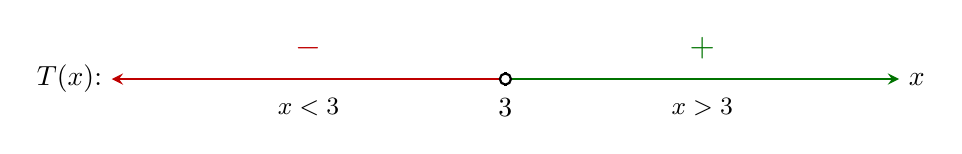
\begin{tikzpicture}[x=1cm,y=1cm,>=stealth]
\draw[<-,thick,red!75!black] (0,0)--(5,0);\draw[->,thick,green!45!black] (5,0)--(10,0);
\draw[black,thick] (5,-0.09)--(5,0.09);\draw[fill=white,thick] (5,0) circle(2pt);
\node[below] at (5,-0.12) {$3$};
\node[above,red!75!black] at (2.5,0.13) {\large $-$};\node[above,green!45!black] at (7.5,0.13) {\large $+$};
\node[left] at (0,0) {$T(x)$:};\node[right] at (10,0) {$x$};
\node[below] at (2.5,-0.12) {\small $x<3$};\node[below] at (7.5,-0.12) {\small $x>3$};
\end{tikzpicture}
\end{center}
Pavyzdžiui, $T(2)=-1<0$, o $T(5)=2>0$. Visų kitų intervalo taškų ženklą pagrindžia aukščiau pateiktas palyginimas su $3$, o ne vien šie du skaičiavimai.

\medskip
\textbf{Ką dar svarbu žinoti apie brėžinius?}
\begin{itemize}[leftmargin=*,itemsep=1pt,topsep=2pt]
\item Tolesniuose brėžiniuose spalvos padeda atpažinti ženklą, bet juo laikome $+$ arba $-$ simbolį.
\item Ženklas virš intervalo galioja visam intervalui, o tuščiaviduriame taške reiškinys lygus $0$, todėl nėra nei teigiamas, nei neigiamas.
\item Brėžiniai nubraižyti ne pagal mastelį.
\end{itemize}

\textbf{Kaip užrašome intervalus ir sprendinių aibes?}
\begin{itemize}[leftmargin=*,itemsep=1pt,topsep=2pt]
\item Atviri intervalo galai rašomi apvaliaisiais skliaustais, pavyzdžiui, $(2;5)$, o įtraukti galai – laužtiniais: $[2;5]$ reiškia $2\le x\le5$.
\item Sprendinių aibės brėžinyje įtrauktas galas žymimas pilnaviduriu tašku, neįtrauktas – tuščiaviduriu. Pavyzdžiui, $x\ge2$ sprendiniuose taškas $2$ įtraukiamas, o $x>2$ – ne.
\item Ženklai $\pm\infty$ nėra skaičiai, todėl šalia jų visada rašome apvaliuosius skliaustus.
\end{itemize}
\needspace{4.5cm}
\begin{enumerate}[series=uzdaviniai]
\item Nagrinėkite reiškinį $x-2$.
\begin{enumerate}
\item Apskaičiuokite jo reikšmes, kai $x=-1$, $x=2$, $x=5$.
\item Paaiškinkite, kodėl $x-2<0$, kai $x<2$; kodėl jis lygus nuliui, kai $x=2$; kodėl $x-2>0$, kai $x>2$.
\item Nubraižykite skaičių tiesę ir pažymėkite ženklus.
\end{enumerate}
\item $\star$ \begin{enumerate}
\item Tegul $t$ yra bet koks realusis skaičius. Kokį ženklą turi $x-t$, kai $x<t$, kai $x=t$ ir kai $x>t$? Paaiškinkite kiekvieną atvejį.
\item Pritaikykite išvadą reiškiniams $x+3$ ir $x-5$. Su kuria $x$ reikšme kiekvienas iš jų lygus $0$? Kokį ženklą jie turi kairėje ir dešinėje nuo tos reikšmės?
\end{enumerate}
\item Duotas $P(x)=(x-1)(x-4)$. Šiame uždavinyje tirsime, kaip kinta $P(x)$ ženklas. Skaičių tiesėje pažymėtos reikšmės $x=1$ ir $x=4$, su kuriomis vienas iš dauginamųjų lygus $0$; jos padalija tiesę į tris intervalus.
\paruosiamojitiese{1}{4}
\begin{enumerate}
\item Užrašykite tris intervalus, į kuriuos taškai $1$ ir $4$ padalija skaičių tiesę.
\item Kiekviename intervale nustatykite dauginamųjų $x-1$ ir $x-4$ ženklus ir pagal sandaugos ženklų taisyklę nustatykite $P(x)$ ženklą.
\item Atskirai nustatykite $P(1)$ ir $P(4)$. Apskaičiuokite $P(0)$, $P(2)$ ir $P(5)$ ir palyginkite su ženklais, kuriuos gavote b dalyje.
\item Nubraižykite $P(x)$ ženklų tiesę ir atsakykite, kur $P(x)>0$, kur $P(x)<0$, o kur $P(x)=0$.
\end{enumerate}
\item Tegul $P(x)=-(x-1)(x-4)$.
\begin{enumerate}
\item Pasinaudodami 3 uždaviniu paaiškinkite, kaip dauginimas iš $-1$ pakeičia ženklą. Ką gauname, kai $x=1$ ir kai $x=4$?
\item Nustatykite ir skaičių tiesėje pažymėkite, kur $P(x)>0$, kur $P(x)<0$ ir kur $P(x)=0$.
\end{enumerate}
\item $\star$ Tegul $r<s$ ir $P(x)=a(x-r)(x-s)$, $a\ne0$.
\paruosiamojitiese{r}{s}
\begin{enumerate}
\item Kiekviename intervale $(-\infty;r)$, $(r;s)$, $(s;+\infty)$ nustatykite $x-r$ ir $x-s$ ženklus. Koks yra jų sandaugos ženklas?
\item Remdamiesi a dalimi išnagrinėkite $P(x)$ ženklus, kai $a>0$, ir juos pavaizduokite skaičių tiesėje.
\item Tą patį padarykite, kai $a<0$. Atskirai nurodykite, ką gauname ties $x=r$ ir $x=s$.
\item Kodėl užrašant intervalą $(r;s)$ reikia sąlygos $r<s$? Kas pasikeistų, jei būtų $r>s$?
\end{enumerate}
\par\medskip
\textbf{Sustok ir apibendrink.} Kaip pagal dauginamųjų ženklus nustatyti $a(x-r)(x-s)$ ženklą kiekviename intervale? Ką žinome šaknyse?
\item Kiekvienam daugianariui nubraižykite ženklų tiesę ir nurodykite, kur jo reikšmės teigiamos, neigiamos ar lygios nuliui.
\begin{enumerate}
\item $P(x)=3(x+2)(x-1)$; \item $Q(x)=-2(x-3)(x+1)$; \item $R(x)=(x+4)(x+2)$; \item $S(x)=-x(x-5)$.
\end{enumerate}
\needspace{3.5cm}
\item Kiekvienu atveju pirmiausia raskite šaknis, išskaidykite daugianarį ir pagal dauginamųjų ženklus nustatykite jo ženklą. Pavaizduokite ženklų tiesę.
\begin{multicols}{2}\begin{enumerate}
\item $x^2-5x+6$; \item $-x^2+x+6$; \item $2x^2-8x-10$; \item $-x^2-4x$.
\end{enumerate}\end{multicols}
\item Duotas $P(x)=(x-2)^2$.
\begin{enumerate}
\item Kodėl $P(x)\geq0$ kiekvienam $x$? Kada $P(x)=0$?
\item Įrodykite, kad kai $x\ne2$, $P(x)>0$. Palyginkite $P(x)$ ženklus, kai $x<2$ ir kai $x>2$. Kam lygus $P(2)$?
\item Pavaizduokite ženklų tiesę ir palyginkite ją su 3 uždavinio ženklų tiese.
\end{enumerate}
\item $\star$ Tegul $P(x)=a(x-r)^2$, $a\ne0$.
\begin{enumerate}
\item Nustatykite $P(r)$ ir paaiškinkite, kodėl $(x-r)^2>0$, kai $x\ne r$.
\item Nubraižykite ženklų tieses, kai $a>0$ ir kai $a<0$. Palyginkite ženklus, kai $x<r$ ir kai $x>r$. Kam lygus $P(r)$?
\end{enumerate}
\par\medskip
\textbf{Sustok ir apibendrink.} Kaip skiriasi ženklai abipus dvigubosios šaknies? Kokia reikšmė yra pačioje šaknyje?
\item Kiekvienu atveju raskite šaknį, užrašykite pilnojo kvadrato pavidalą ir nustatykite ženklą visoje skaičių tiesėje.
\begin{enumerate}
\item $x^2-6x+9$; \item $-2x^2-8x-8$; \item $4x^2$.
\end{enumerate}
\item Duotas $P(x)=(x-1)^2+3$.
\begin{enumerate}
\item Paaiškinkite, kodėl $(x-1)^2\geq0$. Pridėję po $3$ prie abiejų nelygybės pusių, įrodykite, kad $P(x)\geq3>0$.
\item Ar $P$ turi realiųjų šaknų? Pavaizduokite jo ženklą skaičių tiesėje.
\item Nustatykite $Q(x)=-2(x+1)^2-5$ ženklą ir paaiškinkite savo išvadą.
\end{enumerate}
\item $\star$ Tegul $P(x)=ax^2+bx+c$, $a\ne0$, ir $D<0$. Iš 4 temos 2 uždavinio žinome tapatybę
\[P(x)=a\left(x+\frac{b}{2a}\right)^2-\frac{D}{4a}.\]
\begin{enumerate}
\item Kodėl, kai $D<0$, daugianaris neturi realiųjų šaknų?
\item Tarkime, $a>0$. Nustatykite $-\frac{D}{4a}$ ženklą ir įrodykite, kad $P(x)>0$ kiekvienam realiajam $x$.
\item Tą patį padarykite, kai $a<0$. Palyginkite daugianario ženklą su $a$ ženklu.
\end{enumerate}
\par\medskip
\textbf{Sustok ir apibendrink.} Kodėl, kai $D<0$, daugianario ženklas visur sutampa su $a$ ženklu?
\item Nustatykite daugianario ženklą visoje skaičių tiesėje ir kiekvieną išvadą pagrįskite.
\begin{enumerate}
\item $x^2+2x+5$; \item $-x^2+4x-7$; \item $2x^2+2$.
\end{enumerate}
\item Kiekvienu atveju nustatykite $D$ ženklą, šaknis, jei jų yra, ir daugianario ženklą kiekviename intervale. Nubraižykite ženklų tiesę.
\begin{enumerate}
\item $x^2-4x+3$; \item $x^2-4x+4$; \item $x^2-4x+5$; \item $-x^2+4x-3$.
\end{enumerate}
\item Mokinys teigia: „Kvadratinio daugianario ženklai kairėje ir dešinėje kiekvienos šaknies pusėse yra skirtingi.“ Ar teiginys teisingas? Palyginkite $P(x)=(x-1)(x-3)$ ir $Q(x)=(x-2)^2$; nubraižykite abi ženklų tieses.
\item Duota, kad kvadratinio daugianario $P(x)$ šaknys yra $-2$ ir $4$, o $P(0)=8$.
\begin{enumerate}
\item Užrašykite $P(x)$ sandaugos pavidalu ir raskite $a$.
\item Nustatykite $P$ ženklą visoje skaičių tiesėje. Raskite ekstremumo tašką ir ekstremumo reikšmę.
\item Paaiškinkite, kodėl šių duomenų pakanka vienam daugianariui nustatyti.
\end{enumerate}
\item Tarkime, kvadratinio daugianario $P(x)$ minimumas yra $-4$, o minimumo taškas $x=3$; be to, $P(1)=4$.
\begin{enumerate}
\item Užrašykite $P(x)$ pilnojo kvadrato pavidalu su nežinomu $a$ ir, naudodamiesi $P(1)=4$, raskite $a$.
\item Raskite šaknis ir sandaugos pavidalą.
\item Nustatykite ženklą visoje skaičių tiesėje ir patikrinkite duotas sąlygas.
\end{enumerate}
\item $\star$ Mokinys sako: „Kadangi $P(0)>0$ ir $P(5)>0$, tai $P(x)>0$ visiems $x$ tarp $0$ ir $5$.“ Nagrinėkite $P(x)=(x-1)(x-4)$.
\begin{enumerate}
\item Apskaičiuokite $P(0)$, $P(5)$ ir $P(2)$. Ar mokinio išvada teisinga?
\item Pažymėkite skaičių tiesėje taškus $0$, $1$, $4$, $5$. Ar šaknys $1$ ir $4$ yra tarp $0$ ir $5$? Į kiek dalių jos suskaido intervalą $(0;5)$ ir kodėl vien reikšmių $P(0)$ ir $P(5)$ nepakanka daryti išvadą apie visą šį intervalą?
\item Kodėl kiekviename iš intervalų $(-\infty;1)$, $(1;4)$, $(4;+\infty)$ daugianario $P(x)$ ženklas pastovus?
\item Kodėl tada kiekvieno tokio intervalo ženklui nustatyti pakanka vieno jame pasirinkto taško?
\end{enumerate}
\par\medskip
\textbf{Sustok ir apibendrink.} Kada intervalo ženklą galima nustatyti pagal vieną jo tašką? Kodėl dviejų teigiamų reikšmių (kaip $P(0)$ ir $P(5)$) neužtenka?
\item Kvadratinio daugianario $P(x)$ ženklų tiesė yra tokia, o $P(0)=-8$:
\dutaske{1}{4}{-}{+}{-}
\begin{enumerate}
\item Ką iš brėžinio galite pasakyti apie šaknis ir vyriausiojo koeficiento ženklą?
\item Užrašykite $P(x)$ sandaugos pavidalu ir, naudodamiesi $P(0)$, raskite vyriausiąjį koeficientą.
\item Užrašykite standartinį ir pilnojo kvadrato pavidalus. Patikrinkite ženklus ir duotą reikšmę.
\end{enumerate}
\item Kvadratinio daugianario $P(x)$ ženklų tiesė yra
\dutaske{-2}{2}{+}{-}{+}
o jo minimumas lygus $-8$.
\begin{enumerate}
\item Raskite šaknis, ekstremumo tašką ir užrašykite $P(x)$ per vyriausiąjį koeficientą $a$.
\item Iš minimumo raskite $a$, tada užrašykite $P(x)$ visais trimis pavidalais.
\item Patikrinkite ženklų tiesę ir minimumą. Kodėl šie duomenys nusako tik vieną daugianarį?
\end{enumerate}
\needspace{4cm}
\item Kvadratinio daugianario $P(x)$ ženklų tiesė yra
\dutaske{1}{5}{+}{-}{+}
o $P(2)=-6$. Raskite $P(x)$, jo ekstremumo tašką ir ekstremumą. Patikrinkite atsakymą.
\item Kvadratinio daugianario $P(x)$ ženklų tiesė yra
\dutaske{-1}{3}{-}{+}{-}
o diskriminantas lygus $64$. Raskite visus tokius daugianarius.
\begin{enumerate}
\item Užrašykite $P(x)$ per $a$ ir išreikškite $D$ per $a$ (galite remtis šaknų formule arba ryšiu $D=a^2(x_1-x_2)^2$).
\item Raskite $a$, panaudodami ženklų tiesę, ir patikrinkite gautą rezultatą.
\end{enumerate}
\item Kvadratinio daugianario $P(x)$ ženklų tiesė rodo, kad $P(x)>0$ su visomis $x$ reikšmėmis (šaknų nėra):
\visaaxis{+}
Žinoma, kad minimumo taškas yra $x=2$, minimumas yra $3$, o $P(0)=11$. Raskite $P(x)$ standartiniu ir pilnojo kvadrato pavidalais. Ar jis turi realiųjų šaknų? Patikrinkite visas sąlygas.
\item Kvadratinio daugianario ženklų tiesė yra tokia:
\vientaske{2}{+}{+}
Be to, $P(0)=12$. Raskite $P(x)$, jo diskriminantą ir ekstremumą. Patikrinkite, kad atsakymas tenkina ir ženklų tiesėje pateiktą informaciją.
\item Kvadratinis daugianaris $P(x)$ yra teigiamas tik intervale $(1;3)$, o $P(1)=P(3)=0$. Jo maksimumas lygus $4$. Raskite $P(x)$ ir nubraižykite ženklų tiesę. Paaiškinkite, kodėl iš sąlygų pakanka duomenų vienam daugianariui rasti.
\item Ar egzistuoja kvadratinis daugianaris, kuris būtų teigiamas visiems realiesiems $x$, o jo diskriminantas būtų lygus $4$? Atsakymą pagrįskite.
\item Raskite \emph{visus} kvadratinius daugianarius $P(x)=ax^2+bx+c$, kurie yra teigiami kiekvienam realiajam $x$ ir tenkina $P(0)=1$.
\begin{enumerate}
\item Ką apie $c$, $a$ ir diskriminantą pasako sąlygos?
\item Užrašykite, kokias sąlygas turi tenkinti $a$ ir $b$, kai $c=1$, ir pagrįskite, kad jų pakanka.
\item Pateikite du skirtingus tokius daugianarius. Ar žinomos informacijos pakanka vienam daugianariui nustatyti?
\end{enumerate}
\item Kiekvienu atveju nustatykite visas realiąsias $x$ reikšmes, tenkinančias atitinkamą nelygybę, ir pavaizduokite sprendinių aibes skaičių tiesėje. Įtrauktą reikšmę žymėkite pilnaviduriu, neįtrauktą – tuščiaviduriu tašku.
\begin{enumerate}
\item $(x-1)(x-4)>0$; \item $(x-1)(x-4)\ge0$; \item $(x-1)(x-4)\le0$; \item $(x-2)^2\le0$.
\end{enumerate}
Paaiškinkite, kodėl a)–d) dalyse vienose šaknys įtraukiamos, o kitose – ne.
\item \textbf{Grįžkime prie kurso pradžios.} Duotas $P(x)=x^2-4x+3$.
\begin{enumerate}
\item Kada $P(x)=0$? Paaiškinkite, kaip tai susiję su šaknimis.
\item Kada $P(x)>0$, kada $P(x)<0$, o kada $P(x)\ge0$? Ženklų ir sprendinių tiesėse pažymėkite taškus pagal jų įtraukimą.
\item Raskite ekstremumo tašką ir ekstremumą. Ką jie sako apie visas daugianario reikšmes?
\item Ar vien sąlygų $P(1)=P(3)=0$ ir $P(0)=3$ pakanka, kad daugianaris būtų būtent $x^2-4x+3$? Pagrįskite.
\item Kurių ankstesnių temų išvadomis naudojotės? Savais žodžiais apibendrinkite, kaip atsakytumėte į a)–d) klausimus apie kitą kvadratinį daugianarį.
\end{enumerate}
\item \textbf{Papildomas iššūkis.} Raskite realųjį $m$, su kuriuo lygtis $x^2-mx+m=0$ turi realiųjų šaknų, o jų kvadratų suma yra mažiausia. Vienintelės šaknies atveju laikykite $x_1=x_2$. Nurodykite, kokios $m$ reikšmės leistinos, ir pagrįskite, kad rastoji reikšmė yra mažiausia.
\end{enumerate}
\newpage
\begin{center}{\Large\bfseries Ką atradome?}\end{center}
Prieš skaitydamas, pabandyk pats prisiminti ir savais žodžiais paaiškinti pagrindines šios temos išvadas. Tada palygink jas su pateiktomis.
\begin{tcolorbox}[title=Svarbiausios temos išvados,colback=black!3,colframe=black!65,boxrule=0.6pt,arc=2mm]
\begin{enumerate}
\item \textbf{Ženklų tiesė.} $+$ virš intervalo reiškia $P(x)>0$ su kiekviena jo $x$ reikšme, o $-$ reiškia $P(x)<0$. Šaknyje $P(x)=0$, o skaičius $0$ nėra nei teigiamas, nei neigiamas. Sprendinių tiesėje įtrauktas taškas yra pilnaviduris, neįtrauktas – tuščiaviduris; ženklų tiesėje tuščiavidurės šaknys neįeina į griežto ženklo intervalus, nes jose reikšmė lygi $0$.
\item \textbf{Dvi šaknys.} Kai $r<s$ ir $P(x)=a(x-r)(x-s)$, sandauga $(x-r)(x-s)$ teigiama intervaluose $(-\infty;r)$ ir $(s;+\infty)$, o intervale $(r;s)$ neigiama. Jei $a<0$, ženklai pasikeičia į priešingus; šaknyse reikšmė lygi nuliui.
\item \textbf{Viena šaknis.} Kai $P(x)=a(x-r)^2$, tai $P(r)=0$, o su kiekvienu $x\ne r$ jo ženklas sutampa su $a$ ženklu. Abipus šaknies ženklai vienodi.
\item \textbf{Šaknų nėra.} Kai $D<0$, visoms realiosioms $x$ reikšmėms $P(x)$ ženklas sutampa su $a$ ženklu. Tai pagrindžia pilnojo kvadrato pavidalas.
\item \textbf{Kaip tirti?} Nustatyk šaknis ir jų tvarką; skaidyk, jei realiųjų šaknų yra; išnagrinėk dauginamųjų ženklus intervaluose; atskirai nurodyk reikšmes šaknyse. Kai ženklas intervale jau pagrįstai pastovus, jį galima nustatyti pasirinkus vieną to intervalo tašką. Sprendžiant $P(x)\ge0$ ar $P(x)\le0$, į sprendinius įtraukiamos ir šaknys; sprendžiant griežtą nelygybę jos neįtraukiamos.
\end{enumerate}
\end{tcolorbox}
\textbf{Kas toliau?} Vėliau šaknis, ekstremumą, simetriją ir ženklus galėsite susieti su jų geometriniu vaizdu.

\textbf{Ką verta užsirašyti savo teorijos santraukoje?} Pasirink svarbią išvadą ir užsirašyk faktą, jo sąlygas, kodėl jis teisingas, ir vieną savo pavyzdį. Išvadų taikymą pasitikrink toliau pateiktu $\blacklozenge$ pažymėtu uždaviniu.
\newpage
\begin{center}{\Large\bfseries Savikontrolė}\end{center}
Pirmiausia užversk teorijos santrauką ir savarankiškai išspręsk uždavinį. Pasitikrink atsakymus, o jei kuri nors dalis kėlė sunkumų, grįžk prie atitinkamos išvados ir pabandyk dar kartą. Kitą dieną dar kartą išspręsk šį uždavinį nesinaudodamas santrauka.
\begin{enumerate}[resume=uzdaviniai]
\item $\blacklozenge$ Atlikite užduotis ir pagrįskite atsakymus.
\begin{enumerate}
\item Raskite $P(x)=2x^2+2x-12$ šaknis, nustatykite ženklą kiekviename intervale ir nubraižykite ženklų tiesę.
\item Nustatykite $Q(x)=-3(x-1)^2$ ženklą visoje skaičių tiesėje. Kam lygus $Q(1)$?
\item Pagrįskite, koks yra $R(x)=-(x-2)^2-1$ ženklas su visomis realiosiomis $x$ reikšmėmis.
\item Raskite kvadratinį daugianarį, kurio šaknys yra $-2$ ir $3$, ženklų tiesėje tarp šaknų yra $-$, o $P(0)=-12$. Patikrinkite visas sąlygas.
\end{enumerate}
\end{enumerate}
\newpage
\begin{center}{\Large\bfseries Atsakymai ir sprendimai}\end{center}
\begin{enumerate}
\item \textbf{a)} Kai $x=-1$, gauname $-3$; kai $x=2$, gauname $0$; kai $x=5$, gauname $3$.

\textbf{b)} Jei $x<2$, atėmę $2$ iš abiejų nelygybės pusių gauname $x-2<0$. Kai $x=2$, $x-2=0$. Jei $x>2$, analogiškai $x-2>0$.

\textbf{c)} Reiškinio $x-2$ ženklų tiesė:
\vientaske{2}{-}{+}
\item \textbf{a)} Atėmę $t$ iš abiejų pusių, gauname: kai $x<t$, $x-t<0$; kai $x=t$, $x-t=0$; kai $x>t$, $x-t>0$.

\textbf{b)} Kadangi $x+3=x-(-3)$, jis lygus $0$, kai $x=-3$: kai $x<-3$, jis neigiamas, kai $x>-3$, teigiamas. $x-5$ lygus $0$, kai $x=5$: kai $x<5$, jis neigiamas, kai $x>5$, teigiamas.
\item \textbf{a)} Gauname intervalus $(-\infty;1)$, $(1;4)$, $(4;+\infty)$.

\textbf{b)} Jei $x<1$, abu dauginamieji neigiami, todėl sandauga teigiama. Jei $1<x<4$, pirmasis teigiamas, antrasis neigiamas, todėl sandauga neigiama. Jei $x>4$, abu teigiami, todėl sandauga teigiama.

\begin{center}
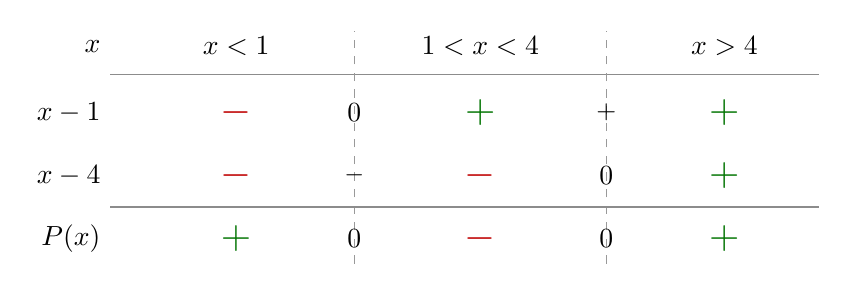
\begin{tikzpicture}[x=1cm,y=0.8cm]
\node[left] at (0,2.3) {$x$}; \node at (1.6,2.3) {$x<1$}; \node at (4.7,2.3) {$1<x<4$}; \node at (7.8,2.3) {$x>4$};
\draw[black!45] (0,1.85)--(9,1.85); \draw[dashed,black!40] (3.1,-1.15)--(3.1,2.55);\draw[dashed,black!40] (6.3,-1.15)--(6.3,2.55);
\node[left] at (0,1.25) {$x-1$}; \node at (1.6,1.25) {\zenklas{-}};\node at (3.1,1.25) {$0$};\node at (4.7,1.25) {\zenklas{+}};\node at (6.3,1.25) {\small $+$};\node at (7.8,1.25) {\zenklas{+}};
\node[left] at (0,0.25) {$x-4$}; \node at (1.6,0.25) {\zenklas{-}};\node at (3.1,0.25) {\small $-$};\node at (4.7,0.25) {\zenklas{-}};\node at (6.3,0.25) {$0$};\node at (7.8,0.25) {\zenklas{+}};
\draw[black!45] (0,-0.25)--(9,-0.25);
\node[left] at (0,-0.75) {$P(x)$}; \node at (1.6,-0.75) {\zenklas{+}};\node at (3.1,-0.75) {$0$};\node at (4.7,-0.75) {\zenklas{-}};\node at (6.3,-0.75) {$0$};\node at (7.8,-0.75) {\zenklas{+}};
\end{tikzpicture}
\end{center}
\textbf{c)} $P(1)=P(4)=0$. Patikra: $P(0)=(-1)(-4)=4>0$, $P(2)=1\cdot(-2)=-2<0$, $P(5)=4\cdot1=4>0$. Šios reikšmės patvirtina b dalyje gautus ženklus: $P(0)>0$, $P(2)<0$, $P(5)>0$.

\textbf{d)}
\dutaske{1}{4}{+}{-}{+}
$P(x)>0$, kai $x\in(-\infty;1)\cup(4;+\infty)$; $P(x)<0$, kai $x\in(1;4)$; $P(x)=0$, kai $x=1$ arba $x=4$.
\item \textbf{a)} Dauginant iš $-1$, teigiamas skaičius tampa neigiamu, o neigiamas – teigiamu. Kai $x=1$ ir $x=4$, $P(x)=0$, o $-0=0$, todėl šiose reikšmėse $P(x)$ lieka lygus $0$.

\textbf{b)}
\dutaske{1}{4}{-}{+}{-}
$P(x)>0$ intervale $(1;4)$; $P(x)<0$ intervaluose $(-\infty;1)$ ir $(4;+\infty)$; šaknys $1$, $4$.
\item \textbf{a)} Kai $x<r<s$, abu skirtumai neigiami, sandauga teigiama. Kai $r<x<s$, pirmasis skirtumas teigiamas, antrasis neigiamas, sandauga neigiama. Kai $r<s<x$, abu skirtumai teigiami, sandauga teigiama.

\textbf{b)} Kai $a>0$, daugyba iš $a$ ženklų nekeičia:
\dutaske{r}{s}{+}{-}{+}

\needspace{3.3cm}
\textbf{c)} Kai $a<0$, daugyba iš $a$ visus nenulinius ženklus pakeičia priešingais:
\dutaske{r}{s}{-}{+}{-}
Abiem atvejais $P(r)=P(s)=0$, nes vienas dauginamasis lygus nuliui.

\textbf{d)} Intervalą $(r;s)$ sudaro skaičiai, didesni už $r$ ir mažesni už $s$, todėl jis turi prasmę tik kai $r<s$. Jei būtų $r>s$, intervalas tarp šaknų būtų $(s;r)$, o ženklų tiesėje šaknis reikėtų sukeisti vietomis.
\item \textbf{a)} Šaknys $-2<1$, $a=3>0$:
\dutaske{-2}{1}{+}{-}{+}
$P>0$ išoriniuose intervaluose, $P<0$ intervale $(-2;1)$; ties šaknimis $P=0$.

\textbf{b)} Šaknys $-1<3$, $a=-2<0$:
\dutaske{-1}{3}{-}{+}{-}
$Q>0$ intervale $(-1;3)$; už jo neigiamas; ties šaknimis lygus nuliui.

\textbf{c)} Šaknys $-4<-2$, $a=1>0$:
\dutaske{-4}{-2}{+}{-}{+}
$R<0$ tarp šaknų, teigiamas už jų, lygus nuliui ties šaknimis.

\textbf{d)} Šaknys $0<5$, $a=-1<0$:
\dutaske{0}{5}{-}{+}{-}
$S>0$ tarp šaknų, neigiamas už jų, lygus nuliui ties šaknimis.
\item \textbf{a)} Šaknys $2$, $3$; $P(x)=(x-2)(x-3)$, $a>0$:
\dutaske{2}{3}{+}{-}{+}

\textbf{b)} Šaknys $-2$, $3$; $P(x)=-(x+2)(x-3)$, $a<0$:
\dutaske{-2}{3}{-}{+}{-}

\textbf{c)} $2x^2-8x-10=2(x+1)(x-5)$; šaknys $-1$, $5$, $a>0$:
\dutaske{-1}{5}{+}{-}{+}

\textbf{d)} $-x^2-4x=-x(x+4)$; šaknys $-4$, $0$, $a<0$:
\dutaske{-4}{0}{-}{+}{-}
Kiekviename brėžinyje ženklai galioja atviruose intervaluose, o šaknyse daugianaris lygus nuliui.
\item \textbf{a)} Realaus skaičiaus kvadratas neneigiamas. Kvadratas lygus nuliui tik jei $x-2=0$, t. y. $x=2$.

\textbf{b)} Jei $x\ne2$, tai $x-2\ne0$, todėl $(x-2)^2>0$. Abiejose šaknies pusėse ženklas teigiamas: jis nepasikeičia.

\textbf{c)}
\vientaske{2}{+}{+}
3 uždavinyje ties kiekviena iš dviejų skirtingų šaknų ženklas keitėsi, o čia ties dvigubąja šaknimi nesikeičia.
\item \textbf{a)} $P(r)=a\cdot0^2=0$. Jei $x\ne r$, tai $x-r\ne0$, todėl jo kvadratas teigiamas.

\textbf{b)} Kai $a>0$, visur, išskyrus $r$, sandauga teigiama:
\vientaske{r}{+}{+}
Kai $a<0$, ji visur, išskyrus $r$, neigiama:
\vientaske{r}{-}{-}
Kai $x=r$, yra $P(r)=0$, o skaičius $0$ nėra nei teigiamas, nei neigiamas. Nenulinis daugianario ženklas kairėje ir dešinėje šaknies pusėse yra tas pats.
\item \textbf{a)} $x^2-6x+9=(x-3)^2$; šaknis $3$, kitur reikšmės teigiamos:
\vientaske{3}{+}{+}

\textbf{b)} $-2x^2-8x-8=-2(x+2)^2$; šaknis $-2$, kitur reikšmės neigiamos:
\vientaske{-2}{-}{-}

\textbf{c)} $4x^2=4(x-0)^2$; šaknis $0$, kitur reikšmės teigiamos:
\vientaske{0}{+}{+}
\item \textbf{a)} Kvadratas neneigiamas: $(x-1)^2\geq0$. Pridėję po $3$ gauname $(x-1)^2+3\geq3>0$.

\textbf{b)} Kadangi $P(x)\geq3$, $P(x)$ niekada nelygus $0$, todėl realiųjų šaknų nėra:
\visaaxis{+}

\textbf{c)} $(x+1)^2\geq0$. Padauginę iš $-2$ pakeičiame nelygybės kryptį: $-2(x+1)^2\leq0$. Atėmę po $5$ gauname $Q(x)=-2(x+1)^2-5\leq-5<0$. Taigi $Q$ visur neigiamas.
\visaaxis{-}
\item \textbf{a)} Kadangi $D<0$, pagal 6 temos išvadą realiųjų šaknų nėra.

\textbf{b)} Jei $D<0$ ir $a>0$, tai $-D>0$ ir $4a>0$, todėl $-\frac{D}{4a}>0$. Be to, $\left(x+\frac{b}{2a}\right)^2\geq0$, taigi $a\left(x+\frac{b}{2a}\right)^2\geq0$. Pridėję teigiamą skaičių $-\frac{D}{4a}$ prie abiejų nelygybės pusių, gauname
\[P(x)=a\left(x+\frac{b}{2a}\right)^2-\frac{D}{4a}\geq-\frac{D}{4a}>0.\]
Vadinasi, $P(x)>0$ kiekvienam realiajam $x$.

\textbf{c)} Jei $D<0$ ir $a<0$, tai $-D>0$, $4a<0$, todėl $-\frac{D}{4a}<0$. Kadangi kvadratas neneigiamas, o $a<0$, gauname $a\left(x+\frac{b}{2a}\right)^2\leq0$. Pridėję neigiamą skaičių $-\frac{D}{4a}$ prie abiejų pusių, gauname
\[P(x)=a\left(x+\frac{b}{2a}\right)^2-\frac{D}{4a}\leq-\frac{D}{4a}<0.\]
Taigi, kai $D<0$, daugianario ženklas visoje tiesėje sutampa su $a$ ženklu.
\item \textbf{a)} $x^2+2x+5=(x+1)^2+4\geq4>0$ visiems $x$.
\visaaxis{+}

\textbf{b)} $-x^2+4x-7=-(x-2)^2-3\leq-3<0$ visiems $x$.
\visaaxis{-}

\textbf{c)} $2x^2+2\geq2>0$ visiems $x$.
\visaaxis{+}
\item \textbf{a)} $D=4>0$, šaknys $1$, $3$, $a>0$:
\dutaske{1}{3}{+}{-}{+}

\textbf{b)} $D=0$, dviguboji šaknis $2$, $P(x)=(x-2)^2$:
\vientaske{2}{+}{+}

\textbf{c)} $D=-4<0$, šaknų nėra, $P(x)=(x-2)^2+1>0$:
\visaaxis{+}

\textbf{d)} $D=4>0$, šaknys $1$, $3$, $a<0$:
\dutaske{1}{3}{-}{+}{-}
\item Teiginys klaidingas. Pirmajame pavyzdyje ženklas ties abiem skirtingomis šaknimis pasikeičia:
\dutaske{1}{3}{+}{-}{+}
Antrajame ties dvigubąja šaknimi $2$ ženklas nesikeičia, nors pati reikšmė joje lygi nuliui:
\vientaske{2}{+}{+}
\item \textbf{a)} $P(x)=a(x+2)(x-4)$. Iš $P(0)=-8a=8$ gauname $a=-1$, taigi $P(x)=-(x+2)(x-4)$.

\textbf{b)} $a<0$, todėl ženklų tiesė yra
\dutaske{-2}{4}{-}{+}{-}
Ekstremumo taškas $\frac{-2+4}{2}=1$; $P(1)=-(3)(-3)=9$. Kadangi $a<0$, ekstremumas yra maksimumas, todėl $9$ yra didžiausioji reikšmė.

\textbf{c)} $P(0)=-(2)(-4)=8$. Šaknys nustato sandaugos pavidalą, o $P(0)=8$ nustato tik vieną $a=-1$.
\item \textbf{a)} $P(x)=a(x-3)^2-4$. Iš $P(1)=4a-4=4$ gauname $a=2$, todėl $P(x)=2(x-3)^2-4$.

\textbf{b)} Iš $2(x-3)^2-4=0$ gauname $(x-3)^2=2$, todėl šaknys $3-\sqrt2$ ir $3+\sqrt2$. Sandaugos pavidalas yra $P(x)=2(x-3+\sqrt2)(x-3-\sqrt2)$.

\textbf{c)} $a=2>0$, tad
\dutaske{3-\sqrt2}{3+\sqrt2}{+}{-}{+}
$P(3)=-4$, tai minimumas, nes $2(x-3)^2\geq0$; $P(1)=2\cdot4-4=4$.
\item \textbf{a)} $P(0)=(-1)(-4)=4>0$, $P(5)=4\cdot1=4>0$, bet $P(2)=1\cdot(-2)=-2<0$. Todėl mokinio išvada klaidinga: taškas $2$ yra tarp $0$ ir $5$.

\textbf{b)} Šaknys $1$ ir $4$ yra intervalo $(0;5)$ viduje: $0<1<4<5$. Taigi abi šaknys yra tarp $0$ ir $5$ ir suskaido intervalą $(0;5)$ į tris dalis: $(0;1)$, $(1;4)$, $(4;5)$. Taškai $0$ ir $5$ yra išorinėse dalyse, o ženklas gali keistis kertant šaknis, todėl jų reikšmės nepasako, koks ženklas vidurinėje dalyje $(1;4)$.

\textbf{c)} Kiekviename iš intervalų $(-\infty;1)$, $(1;4)$, $(4;+\infty)$ kiekvieno dauginamojo $x-1$ ir $x-4$ ženklas yra pastovus: pavyzdžiui, kai $1<x<4$, pirmasis visada teigiamas, o antrasis visada neigiamas. Todėl ir jų sandaugos ženklas tame intervale yra pastovus.

\textbf{d)} \emph{Kai pastovumas jau pagrįstas}, bet kuris pasirinktas vienas intervalo taškas parodo viso intervalo ženklą. Pavyzdžiui, $P(0)>0$, $P(2)<0$, $P(5)>0$ leidžia pažymėti atitinkamai $+$, $-$, $+$; ties šaknimis $1$ ir $4$ reikšmė yra $0$.
\dutaske{1}{4}{+}{-}{+}
Vieno taško patikra savaime neįrodo ženklo pastovumo: čia jį pirmiausia pagrindėme išskaidyto kvadratinio daugianario dauginamųjų ženklais.
\item \textbf{a)} Taškuose $x=1$ ir $x=4$ brėžinyje pažymėti tuščiaviduriai taškai, kuriuose daugianaris lygus $0$, taigi tai šaknys. Už šaknų daugianaris neigiamas, o tarp jų teigiamas, todėl $a<0$.

\textbf{b)} Pagal skaidymo formulę $P(x)=a(x-1)(x-4)$. Įrašę $x=0$ gauname $P(0)=4a=-8$, taigi $a=-2$.

\textbf{c)} $P(x)=-2(x-1)(x-4)=-2x^2+10x-8=-2\left(x-\frac{5}{2}\right)^2+\frac{9}{2}$. Kadangi $a=-2<0$, ženklai už šaknų neigiami, tarp jų teigiami; $P(0)=-8$. Šaknų ir $P(0)$ pakanka, kad daugianaris būtų nustatytas tik vienas.
\item \textbf{a)} Šaknys yra $-2$ ir $2$, todėl ekstremumo taškas, t. y. šaknų vidurkis, yra $\frac{-2+2}{2}=0$. Kadangi šaknys skirtingos, $P(x)=a(x+2)(x-2)$; iš ženklų tiesės $a>0$.

\textbf{b)} Minimumas pasiekiamas, kai $x=0$, tad $P(0)=-4a=-8$ ir $a=2$. Trys pavidalai:
\[P(x)=2(x+2)(x-2)=2x^2-8=2(x-0)^2-8.\]

\textbf{c)} $P(0)=-8$ ir, kadangi $2x^2\geq0$, minimumas tikrai yra $-8$. Iš $a>0$ ir šaknų $-2$, $2$ gaunami brėžinyje nurodyti ženklai. Šaknų ir minimumo reikšmės pakanka, kad $a$ būtų nustatytas tik vienas.
\item Brėžinyje nurodytos šaknys $1$ ir $5$, o išoriniai ženklai rodo, kad $a>0$. Todėl $P(x)=a(x-1)(x-5)$. Iš $P(2)=a\cdot1\cdot(-3)=-6$ gauname $a=2$.

Taigi $P(x)=2(x-1)(x-5)=2(x-3)^2-8$. Minimumo taškas yra $3$, minimumas $-8$. Patikra: $P(2)=2-8=-6$, o ženklai yra teigiami už šaknų ir neigiami tarp jų.
\item \textbf{a)} Ženklų tiesė duoda šaknis $-1$ ir $3$ bei $a<0$, todėl $P(x)=a(x+1)(x-3)$. Atskliaudę gauname $b=-2a$, $c=-3a$, taigi
\[D=b^2-4ac=4a^2+12a^2=16a^2.\]

\textbf{b)} Iš $16a^2=64$ turime $a=2$ arba $a=-2$; ženklų tiesė reikalauja $a<0$, todėl $a=-2$. Vienintelis atsakymas yra $P(x)=-2(x+1)(x-3)=-2x^2+4x+6$.

Patikra: $D=4^2-4(-2)\cdot6=64$, šaknys $-1$, $3$, o kai $a<0$, ženklai yra $-\,,+\,,-$, kaip brėžinyje.
\item Pagal ekstremumo duomenis $P(x)=a(x-2)^2+3$, o iš $P(0)=4a+3=11$ gauname $a=2$. Taigi $P(x)=2(x-2)^2+3=2x^2-8x+11$.

Kadangi $2(x-2)^2\geq0$, tai $P(x)\geq3>0$ visiems $x$, todėl šaknų nėra. Minimumas $3$ pasiekiamas, kai $x=2$, o $P(0)=11$. Duomenų pakanka, kad $a$ būtų nustatytas tik vienas, taigi daugianaris vienintelis.
\item Brėžinyje ties $2$ yra vienintelis taškas, kuriame daugianaris lygus $0$, o abiejose pusėse reikšmės teigiamos. Vadinasi, $P(x)=a(x-2)^2$, kur $a>0$. Iš $P(0)=4a=12$ randame $a=3$, todėl $P(x)=3(x-2)^2=3x^2-12x+12$.

$D=(-12)^2-4\cdot3\cdot12=0$. Minimumo taškas $2$, minimumas $0$. Kadangi kvadratas teigiamas, kai $x\ne2$, o $a=3>0$, ženklų tiesė tenkinama; $P(0)=12$.
\item Kadangi $P(1)=P(3)=0$, šaknys yra $1$ ir $3$. Daugianaris teigiamas tarp šaknų, todėl $a<0$ ir $P(x)=a(x-1)(x-3)$. Ekstremumo taškas yra šaknų vidurkis $2$. Iš maksimumo $P(2)=-a=4$ gauname $a=-4$.

Taigi $P(x)=-4(x-1)(x-3)=-4(x-2)^2+4$, o jo ženklų tiesė:
\dutaske{1}{3}{-}{+}{-}
Patikra: $P(1)=P(3)=0$, $P(x)>0$ tik intervale $(1;3)$ ir maksimumas yra $4$. Šaknys ir maksimumas nustato tik vieną $a$, todėl daugiau atsakymų nėra.
\item Tokio daugianario nėra. Jeigu $D=4>0$, pagal šaknų formulę jis turėtų dvi realiąsias šaknis. Kiekvienoje šaknyje daugianario reikšmė lygi $0$, todėl jis negali būti teigiamas \emph{visiems} realiesiems $x$.
\item \textbf{a)} Iš $P(0)=1$ gauname $c=1$. Kadangi daugianaris visur teigiamas, jis neturi realiųjų šaknų, todėl $D<0$. Be to, kai realiųjų šaknų nėra, ženklas sutampa su $a$ ženklu; vadinasi, $a>0$.

\textbf{b)} Kadangi $c=1$, tai $D=b^2-4a$. Visos ieškomos sąlygos yra
\[c=1,\qquad a>0,\qquad b^2<4a.\]
Šių sąlygų taip pat pakanka: kai $a>0$ ir $D<0$, realiųjų šaknų nėra, o daugianaris visoje tiesėje teigiamas; be to, $P(0)=c=1$.

\textbf{c)} Pavyzdžiui, $P(x)=x^2+1$ ir $Q(x)=2x^2+1$. Abu daugianariai teigiami visiems $x$, ir $P(0)=Q(0)=1$. Todėl vienam daugianariui nustatyti sąlygų nepakanka.
\item Šaknys yra $1$ ir $4$. Iš sandaugos ženklų: už šaknų reiškinys teigiamas, tarp jų neigiamas, o abiejose šaknyse lygus nuliui.

\textbf{a)} Kai $(x-1)(x-4)>0$, gauname $x\in(-\infty;1)\cup(4;+\infty)$. Šaknys neįtraukiamos – jos pažymėtos tuščiaviduriais taškais:
\begin{center}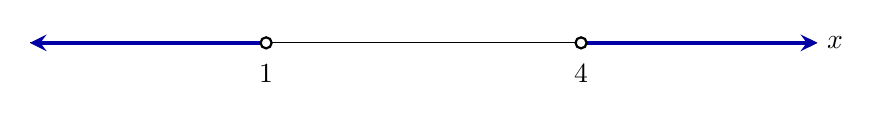
\begin{tikzpicture}[x=1cm,>=stealth]
\draw[->] (0,0)--(10,0) node[right] {$x$};\draw[ultra thick,blue!65!black,->] (3,0)--(0,0);\draw[ultra thick,blue!65!black,->] (7,0)--(10,0);
\draw[fill=white,thick] (3,0) circle(2pt) node[below=4pt] {$1$};\draw[fill=white,thick] (7,0) circle(2pt) node[below=4pt] {$4$};
\end{tikzpicture}\end{center}

\textbf{b)} Kai $(x-1)(x-4)\ge0$, įtraukiame ir abi šaknis: $x\in(-\infty;1]\cup[4;+\infty)$. Jos pažymėtos pilnaviduriais taškais:
\begin{center}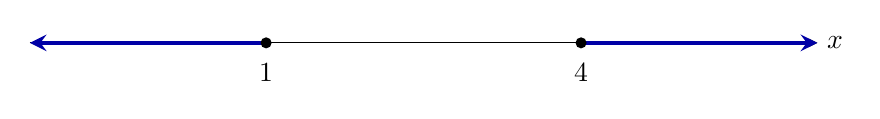
\begin{tikzpicture}[x=1cm,>=stealth]
\draw[->] (0,0)--(10,0) node[right] {$x$};\draw[ultra thick,blue!65!black,->] (3,0)--(0,0);\draw[ultra thick,blue!65!black,->] (7,0)--(10,0);
\fill (3,0) circle(2pt);\fill (7,0) circle(2pt);\node[below=4pt] at (3,0) {$1$};\node[below=4pt] at (7,0) {$4$};
\end{tikzpicture}\end{center}

\textbf{c)} Kai $(x-1)(x-4)\le0$, $P(x)\le0$ yra tarp šaknų ir pačiose šaknyse: $x\in[1;4]$.
\begin{center}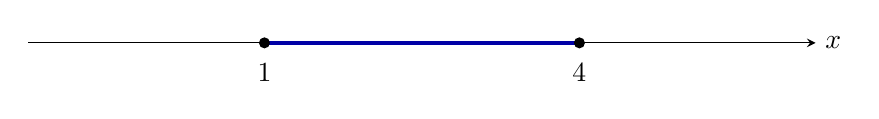
\begin{tikzpicture}[x=1cm,>=stealth]
\draw[->] (0,0)--(10,0) node[right] {$x$};\draw[ultra thick,blue!65!black] (3,0)--(7,0);\fill (3,0) circle(2pt);\fill (7,0) circle(2pt);\node[below=4pt] at (3,0) {$1$};\node[below=4pt] at (7,0) {$4$};
\end{tikzpicture}\end{center}

\textbf{d)} Kadangi $(x-2)^2\ge0$, nelygybė $(x-2)^2\le0$ galima tik tada, kai kvadratas lygus nuliui. Vienintelis sprendinys $x=2$, arba $\{2\}$; taškas įtraukiamas:
\begin{center}\begin{tikzpicture}[x=1cm,>=stealth]
\draw[->] (0,0)--(10,0) node[right] {$x$};\fill[blue!65!black] (5,0) circle(2.5pt);\node[below=4pt] at (5,0) {$2$};
\end{tikzpicture}\end{center}
\item \textbf{a)} $P(x)=(x-1)(x-3)$, todėl šaknys yra $1$ ir $3$ – būtent šios reikšmės tenkina $P(x)=0$.

\textbf{b)} Pagal dauginamųjų ženklus $P(x)>0$, kai $x\in(-\infty;1)\cup(3;+\infty)$; $P(x)<0$, kai $x\in(1;3)$. Pridėję šaknis gauname $P(x)\ge0$, kai $x\in(-\infty;1]\cup[3;+\infty)$. Ženklų tiesėje šaknys tuščiavidurės, nes jose $P(x)=0$, todėl jos neįeina į intervalus, kuriuose $P(x)>0$ ar $P(x)<0$:
\dutaske{1}{3}{+}{-}{+}
O sprendinių $P(x)\ge0$ tiesėje abi šaknys įtrauktos, todėl taškai pilnaviduriai:
\begin{center}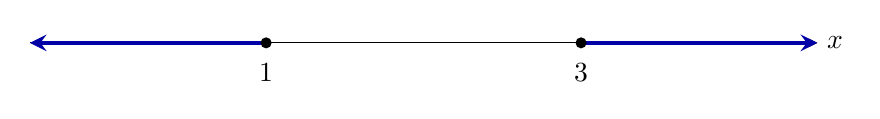
\begin{tikzpicture}[x=1cm,>=stealth]
\draw[->] (0,0)--(10,0) node[right] {$x$};\draw[ultra thick,blue!65!black,->] (3,0)--(0,0);\draw[ultra thick,blue!65!black,->] (7,0)--(10,0);\fill (3,0) circle(2pt);\fill (7,0) circle(2pt);\node[below=4pt] at (3,0) {$1$};\node[below=4pt] at (7,0) {$3$};
\end{tikzpicture}\end{center}

\textbf{c)} $P(x)=(x-2)^2-1\ge-1$. Minimumo taškas $x_{\min}=2$, minimumas $P_{\min}=-1$: visos daugianario reikšmės yra ne mažesnės kaip $-1$, ir ši reikšmė pasiekiama, kai $x=2$.

\textbf{d)} Jei kvadratinio daugianario šaknys $1$ ir $3$, tai $P(x)=a(x-1)(x-3)$. Iš $P(0)=3a=3$ gauname $a=1$ ir daugianaris yra būtent $x^2-4x+3$; tiesioginė patikra duoda $P(1)=P(3)=0$, $P(0)=3$.

\textbf{e)} Šaknų sąvoka ir formulė nagrinėtos 6 temoje, ženklai – šioje temoje, pilnasis kvadratas bei ekstremumas – 2–4 temose, skaidymas ir konstravimas – 9 temoje. Kitam daugianariui pirmiausia pasirenkame patogų pavidalą, apskaičiuojame šaknis ar ekstremumą, atskirai pagrindžiame ženklus ir patikriname, ar duomenų pakanka koeficientams nustatyti.
\item Jei šaknys realiosios, $D=m^2-4m=m(m-4)\ge0$. Ženklų tyrimas duoda $m\in(-\infty;0]\cup[4;+\infty)$: $0$ ir $4$ įtraukiame, nes tada $D=0$ ir yra viena dviguboji šaknis. Pagal Vijeto teoremą $x_1+x_2=m$, $x_1x_2=m$, todėl
\[x_1^2+x_2^2=m^2-2m=(m-1)^2-1.\]
Jei nepaisytume sąlygos $D\ge0$, mažiausią šio reiškinio reikšmę $-1$ gautume, kai $m=1$. Tačiau tada $D=1-4=-3<0$: realiųjų šaknų nėra, todėl $m=1$ nagrinėjamam uždaviniui netinka.

Kai $m\le0$, tai $m^2-2m\ge0$, o lygybė yra tik kai $m=0$. Kai $m\ge4$, tai $m(m-2)\ge4\cdot2=8>0$. Todėl mažiausia kvadratų sumos reikšmė yra $0$, ji pasiekiama vieninteliu atveju $m=0$. Tuomet lygtis $x^2=0$ turi vieną dvigubąją šaknį: $x_1=x_2=0$.
\item \textbf{a)} $2x^2+2x-12=2(x^2+x-6)=2(x+3)(x-2)$. Šaknys yra $-3$ ir $2$. Kai $x<-3$, abu tiesiniai dauginamieji neigiami, todėl sandauga teigiama; kai $-3<x<2$, jų ženklai priešingi, todėl sandauga neigiama; kai $x>2$, abu teigiami. Dauginamasis $2$ teigiamas. Šaknyse reikšmė lygi nuliui:
\dutaske{-3}{2}{+}{-}{+}

\textbf{b)} $(x-1)^2=0$ tik kai $x=1$, o kai $x\ne1$, jis teigiamas. Todėl $Q(1)=0$, o su visomis kitomis reikšmėmis $Q(x)<0$:
\vientaske{1}{-}{-}

\textbf{c)} Kadangi $(x-2)^2\ge0$, tai $-(x-2)^2\le0$. Atėmę $1$ gauname $R(x)\le-1<0$ su visomis realiosiomis $x$ reikšmėmis. Realiųjų šaknų nėra:
\visaaxis{-}

\textbf{d)} Pagal skaidymo formulę $P(x)=a(x+2)(x-3)$, kur $a\ne0$. Iš $P(0)=-6a=-12$ gauname $a=2$, todėl $P(x)=2(x+2)(x-3)=2x^2-2x-12$. Patikra: $P(-2)=P(3)=0$, $P(0)=-12$. Tarp šaknų $x+2>0$, $x-3<0$, o $2>0$, todėl $P(x)<0$. Duomenų pakanka, kad $a$ būtų nustatytas tik vienas.
\end{enumerate}
\end{document}
